\documentclass[a4paper,oneside,12pt]{extreport}

\usepackage{mmap}
\usepackage[T2A]{fontenc}
\usepackage[utf8]{inputenc}
\usepackage[english,russian]{babel}

% Текст отчёта следует печатать, соблюдая следующие размеры полей:
% левое — 30 мм, правое — 15 мм, верхнее и нижнее — 20 мм.
\usepackage[left=20mm, right=15mm, top=15mm, bottom=15mm]{geometry}

% \setlength{\parindent}{1.25cm} % Абзацный отступ

\usepackage{setspace}
% \onehalfspacing % Полуторный интервал

\frenchspacing % Равномерные пробелы
\usepackage{indentfirst} % Красная строка

\usepackage{microtype}
\sloppy

\usepackage{titlesec}
\titlespacing*{\chapter}{0pt}{-30pt}{8pt}
\titlespacing*{\section}{\parindent}{*4}{*4}
\titlespacing*{\subsection}{\parindent}{*4}{*4}
\titleformat{\chapter}{\LARGE\bfseries}{\thechapter}{20pt}{\LARGE\bfseries}
\titleformat{\section}{\Large\bfseries}{\thesection}{40pt}{\Large\bfseries}

\usepackage{graphicx}
\usepackage{caption}

\usepackage[unicode,pdftex]{hyperref}
\hypersetup{hidelinks}

%% title begin
\usepackage{wrapfig}

\makeatletter
	\def\vhrulefill#1{\leavevmode\leaders\hrule\@height#1\hfill \kern\z@}
\makeatother
%% title end

%% begin code
\usepackage{listings}
\usepackage{xcolor}

\lstset{
	basicstyle=\scriptsize\ttfamily,
	breakatwhitespace=true,
	breaklines=true,
	commentstyle=\color{gray},
	frame=single,
	keywordstyle=\color{blue},
	numbers=left,
	numbersep=5pt,
	numberstyle=\tiny\ttfamily\color{gray},
	showstringspaces=false,
	stringstyle=\color{red},
	tabsize=8
}

\lstset{
	literate=
	{а}{{\selectfont\char224}}1 {б}{{\selectfont\char225}}1 {в}{{\selectfont\char226}}1
	{г}{{\selectfont\char227}}1 {д}{{\selectfont\char228}}1 {е}{{\selectfont\char229}}1
	{ё}{{\"e}}1                 {ж}{{\selectfont\char230}}1 {з}{{\selectfont\char231}}1
	{и}{{\selectfont\char232}}1 {й}{{\selectfont\char233}}1 {к}{{\selectfont\char234}}1
	{л}{{\selectfont\char235}}1 {м}{{\selectfont\char236}}1 {н}{{\selectfont\char237}}1
	{о}{{\selectfont\char238}}1 {п}{{\selectfont\char239}}1 {р}{{\selectfont\char240}}1
	{с}{{\selectfont\char241}}1 {т}{{\selectfont\char242}}1 {у}{{\selectfont\char243}}1
	{ф}{{\selectfont\char244}}1 {х}{{\selectfont\char245}}1 {ц}{{\selectfont\char246}}1
	{ч}{{\selectfont\char247}}1 {ш}{{\selectfont\char248}}1 {щ}{{\selectfont\char249}}1
	{ъ}{{\selectfont\char250}}1 {ы}{{\selectfont\char251}}1 {ь}{{\selectfont\char252}}1
	{э}{{\selectfont\char253}}1 {ю}{{\selectfont\char254}}1 {я}{{\selectfont\char255}}1
	{А}{{\selectfont\char192}}1 {Б}{{\selectfont\char193}}1 {В}{{\selectfont\char194}}1
	{Г}{{\selectfont\char195}}1 {Д}{{\selectfont\char196}}1 {Е}{{\selectfont\char197}}1
	{Ё}{{\"E}}1                 {Ж}{{\selectfont\char198}}1 {З}{{\selectfont\char199}}1
	{И}{{\selectfont\char200}}1 {Й}{{\selectfont\char201}}1 {К}{{\selectfont\char202}}1
	{Л}{{\selectfont\char203}}1 {М}{{\selectfont\char204}}1 {Н}{{\selectfont\char205}}1
	{О}{{\selectfont\char206}}1 {П}{{\selectfont\char207}}1 {Р}{{\selectfont\char208}}1
	{С}{{\selectfont\char209}}1 {Т}{{\selectfont\char210}}1 {У}{{\selectfont\char211}}1
	{Ф}{{\selectfont\char212}}1 {Х}{{\selectfont\char213}}1 {Ц}{{\selectfont\char214}}1
	{Ч}{{\selectfont\char215}}1 {Ш}{{\selectfont\char216}}1 {Щ}{{\selectfont\char217}}1
	{Ъ}{{\selectfont\char218}}1 {Ы}{{\selectfont\char219}}1 {Ь}{{\selectfont\char220}}1
	{Э}{{\selectfont\char221}}1 {Ю}{{\selectfont\char222}}1 {Я}{{\selectfont\char223}}1
	{—}{{-}}1
}

\newcommand{\code}[1]{\texttt{#1}}
%% end code

\usepackage{amsmath}


\begin{document}

\begin{titlepage}
	{\large % 14pt instead of 12pt
	\onehalfspacing
	\centering

	\begin{wrapfigure}[7]{l}{0.14\linewidth}
		\vspace{3mm}
		\hspace{-10mm}
		
\includegraphics[width=0.93\linewidth]{inc/img/bmstu-logo}
	\end{wrapfigure}
	{\singlespacing \footnotesize \bfseries Министерство науки и высшего образования Российской Федерации\\Федеральное государственное бюджетное образовательное учреждение\\высшего образования\\<<Московский государственный технический университет\\имени Н.~Э.~Баумана\\ (национальный исследовательский университет)>>\\(МГТУ им. Н.~Э.~Баумана)\\}

	\vspace{-2.2mm}
	\vhrulefill{0.9mm}\\
	\vspace{-7.5mm}
	\vhrulefill{0.2mm}\\
	\vspace{2mm}

	{\doublespacing \small \raggedright ФАКУЛЬТЕТ \hspace{35mm} «Информатика и системы управления»\\
	КАФЕДРА \hspace{15mm} «Программное обеспечение ЭВМ и информационные технологии»\\}

	\vspace{30mm}

	\textbf{ОТЧЁТ}\\
	По лабораторной работе №4\\
	По курсу: «Операционные системы»\\
	Тема: «Виртуальная файловая система /proc»\\

	\vspace{40mm}

	\begin{flushleft}
		\begin{tabular}{lr}
			\textbf{Студент:}        & Керимов~А.~Ш.  \\
			\textbf{Группа:}         & ИУ7-64Б        \\
			\textbf{Преподаватель:}  & Рязанова~Н.~Ю. \\
		\end{tabular}
	\end{flushleft}

	\vfill

	Москва\\
	\the\year\\}
\end{titlepage}

\setcounter{page}{2}


\section*{Часть 1}

\begin{task*}
	Написать приложение по модели клиент-сервер, демонстрирующее взаимодействие параллельных процессов на отдельном компьютере с использованием сокетов в файловом пространстве имен: семейство — \code{AF\_UNIX}, тип — \code{SOCK\_DGRAM}.
	При демонстрации работы программного комплекса необходимо запустить несколько клиентов (не меньше 5) и продемонстрировать, что сервер обрабатывает обращения каждого запущенного клиента.
\end{task*}

\lstinputlisting[caption={\code{unix/socket.h}}\label{lst:unix/socket.h}, language=C]{../unix/socket.h}
\lstinputlisting[caption={\code{unix/server.c}}\label{lst:unix/server.c}, language=C]{../unix/server.c}
\lstinputlisting[caption={\code{unix/client.c}}\label{lst:unix/client.c}, language=C]{../unix/client.c}

\begin{figure}[H]
	\centering
	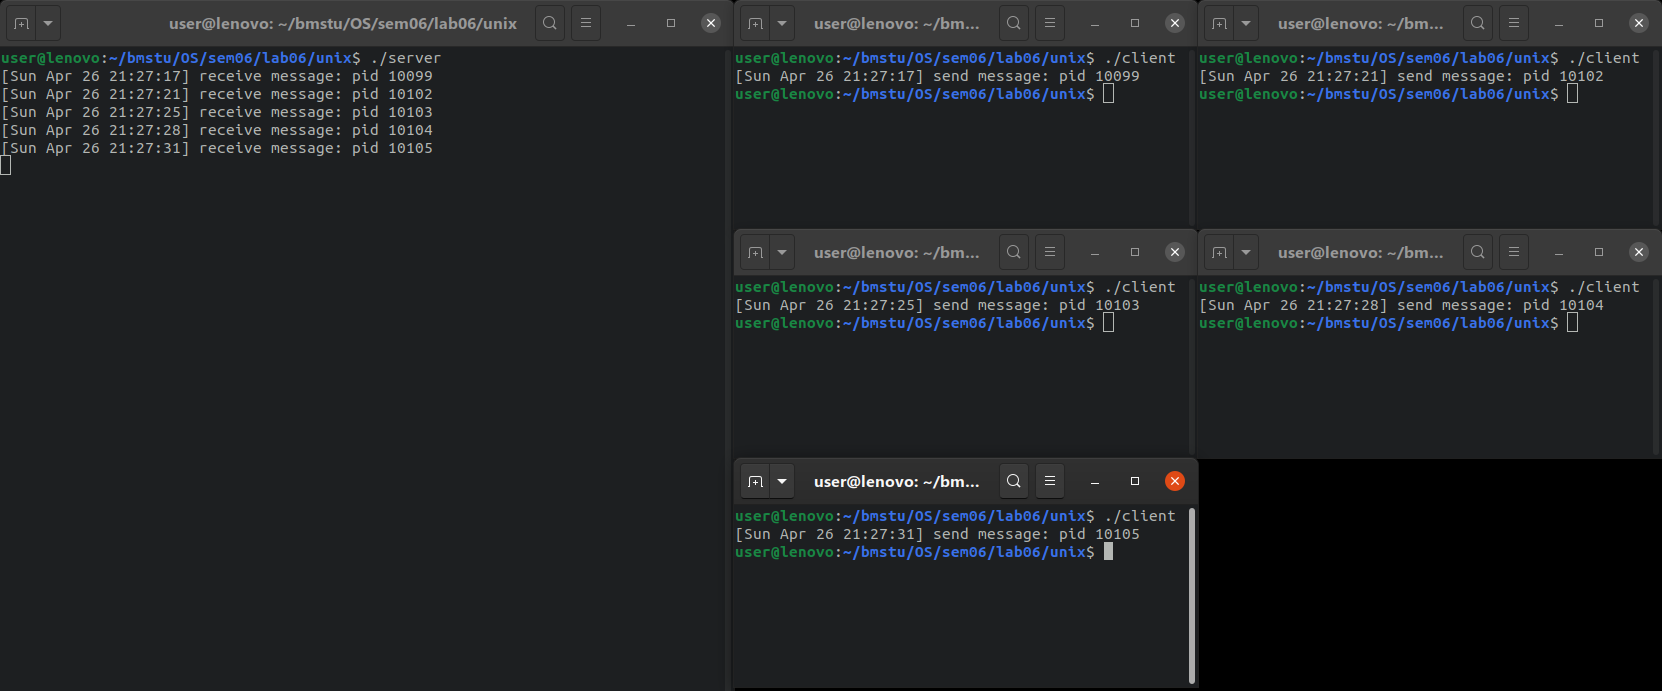
\includegraphics[width=\linewidth]{inc/img/unix-runtime}
	\caption{Демонстрация работы программы}
	\label{img:unix-runtime}
\end{figure}

\section*{Часть 2}

\begin{task*}
	Написать приложение по модели клиент-сервер, осуществляющее взаимодействие параллельных процессов, которые выполняются на разных компьютерах.
	Для взаимодействия с клиентами сервер должен использовать мультиплексирование.
	Сервер должен обслуживать запросы параллельно запущенных клиентов.
	При демонстрации работы программного комплекса необходимо запустить несколько клиентов (не меньше 5) и продемонстрировать, что сервер обрабатывает обращения каждого запущенного клиента.
\end{task*}

\lstinputlisting[caption={\code{net/socket.h}}\label{lst:net/socket.h}, language=C]{../net/socket.h}
\lstinputlisting[caption={\code{net/server.c}}\label{lst:net/server.c}, language=C]{../net/server.c}
\lstinputlisting[caption={\code{net/client.c}}\label{lst:net/client.c}, language=C]{../net/client.c}

\begin{figure}[H]
	\centering
	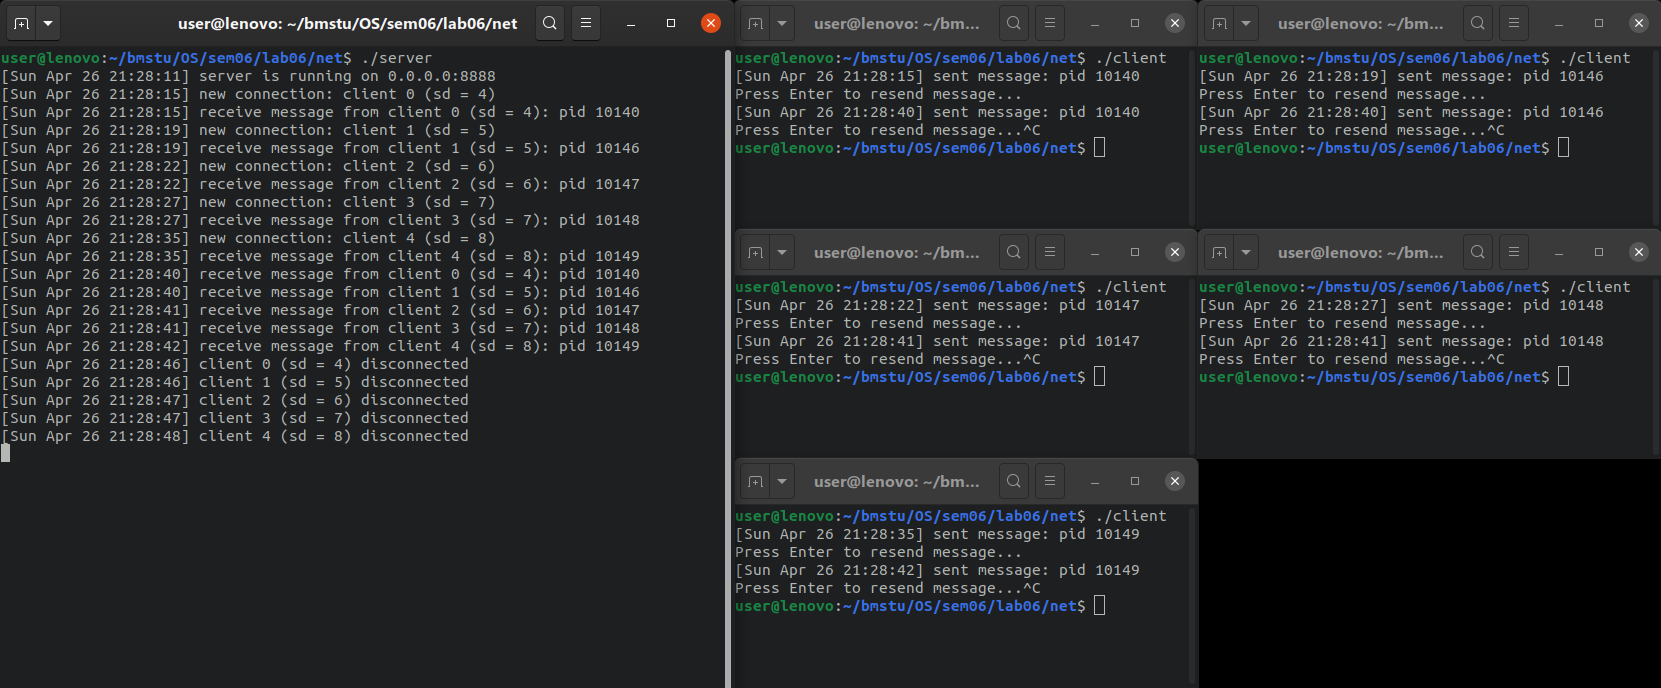
\includegraphics[width=\linewidth]{inc/img/net-runtime}
	\caption{Демонстрация работы программы}
	\label{img:net-runtime}
\end{figure}

\end{document}
